\documentclass[conference]{IEEEtran}
\usepackage{graphicx}
\usepackage{booktabs}
\usepackage{caption}
\usepackage{subcaption}
\usepackage{amsmath,amssymb}
\usepackage{hyperref}
\begin{document}
\title{ML\-AI Motion Controller: Low\-Latency Pose→Game Control with Engineered Features}
\author{Author Name \\ Affiliation}
\maketitle

\begin{abstract}
Paste the paper abstract here (use the Abstract from PAPER_FULL.md).
\end{abstract}

\begin{IEEEkeywords}
pose estimation, feature engineering, MLP, SVM, ST\-GCN, real\-time control
\end{IEEEkeywords}

\section{Introduction}
(Paste Introduction from PAPER_FULL.md)

\section{Related Work}
(Paste Related Work from PAPER_FULL.md)

\section{System Architecture}
\begin{figure}[t]
  \centering
  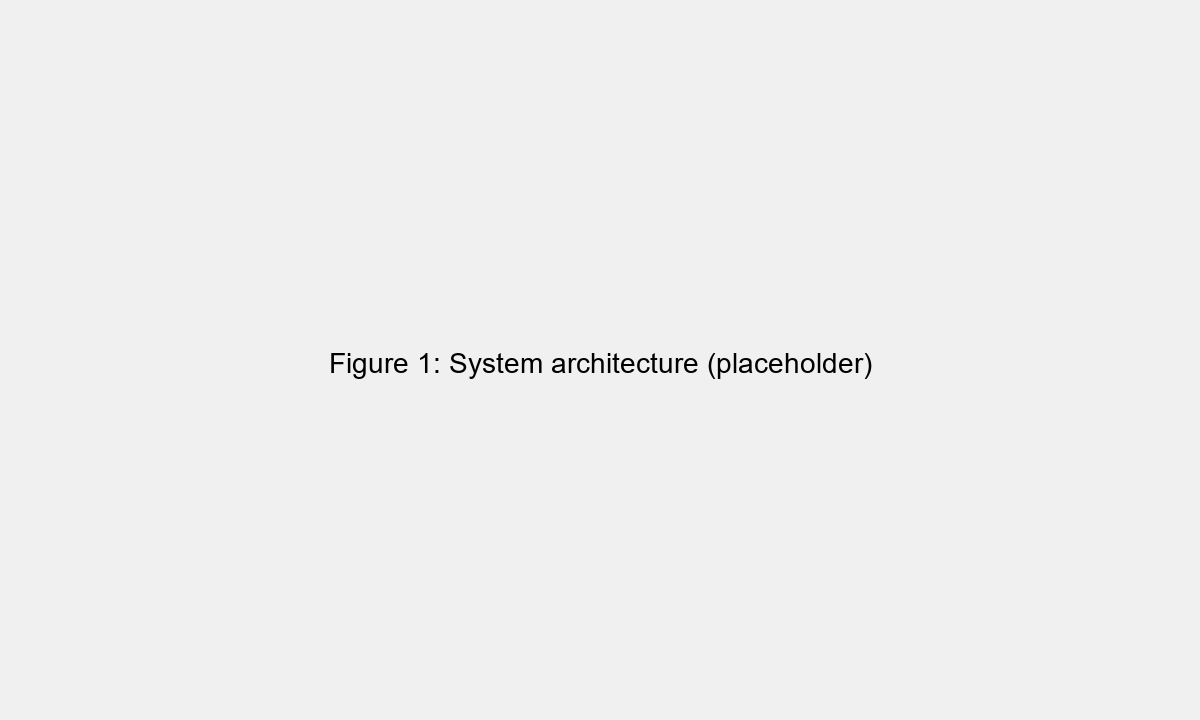
\includegraphics[width=\linewidth]{figs/figure1_system.png}
  \caption{Overall system architecture showing the real\-time pipeline from webcam to game control.}
  \label{fig:system}
\end{figure}

\section{Dataset and Feature Engineering}
\begin{figure}[t]
  \centering
  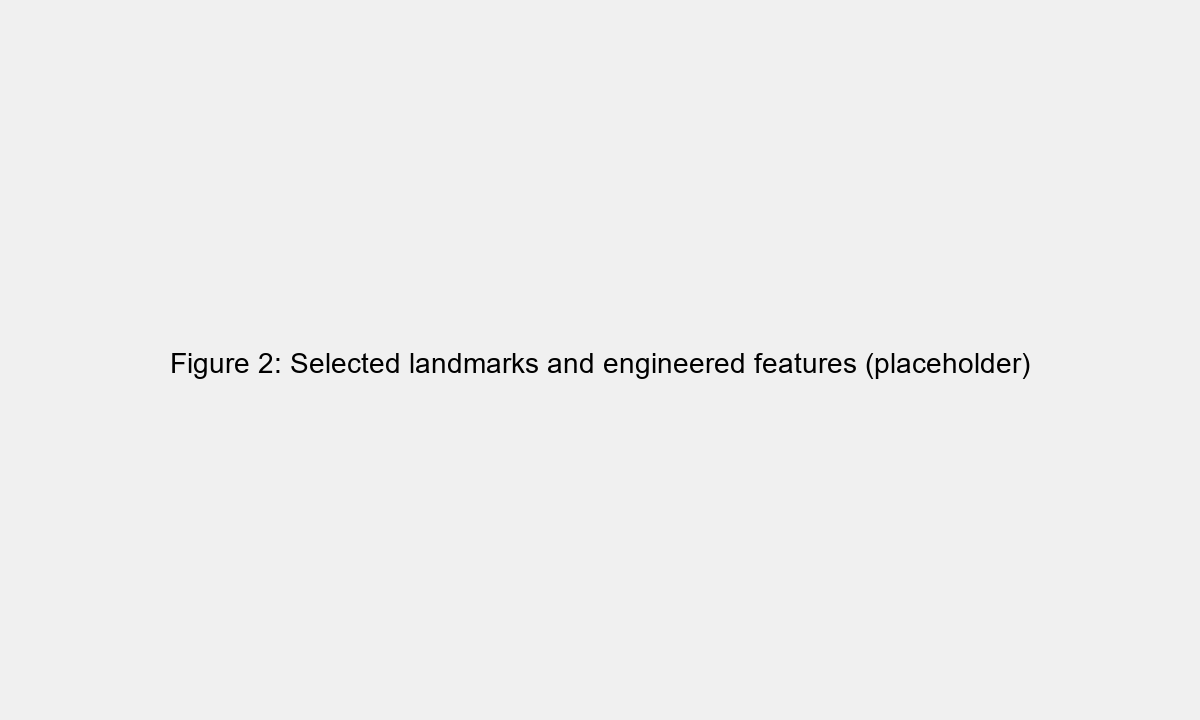
\includegraphics[width=0.9\linewidth]{figs/figure2_landmarks.png}
  \caption{Selected upper\-body landmarks and example engineered features (angles, velocity, acceleration).}
  \label{fig:features}
\end{figure}

\section{Models}
\section{Experiments}
\begin{figure}[t]
  \centering
  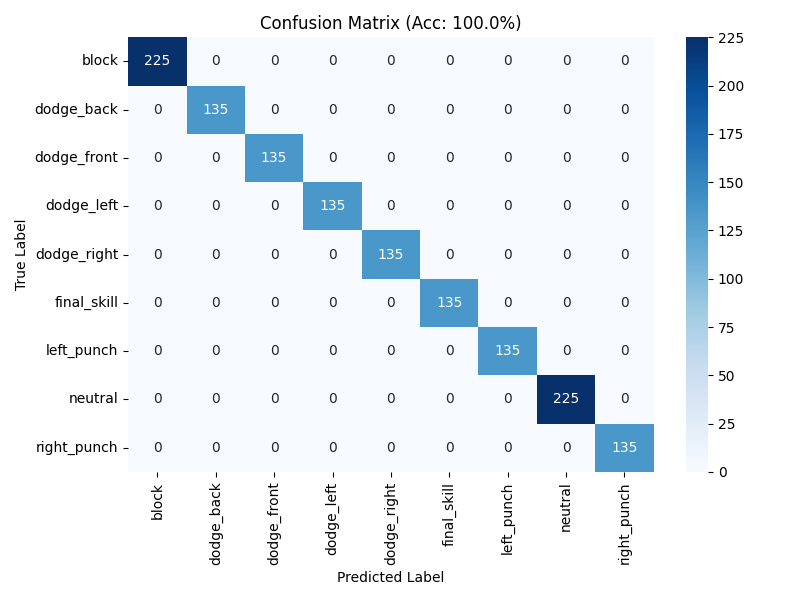
\includegraphics[width=\linewidth]{figs/figure3_confusion.png}
  \caption{Confusion matrix on the held\-out test set for the MLP baseline (95.5\% accuracy).}
  \label{fig:confusion}
\end{figure}

\section{Results}
\begin{table}[t]
  \centering
  \caption{Table 1. Summary of model performance on the held\-out test set (accuracy, macro\-F1, inference latency).}
  \begin{tabular}{lccc}
    \toprule
    Model & Accuracy & Macro\-F1 & Latency (ms) \\
    \midrule
    SVM & 95.0\% & 0.944 & 0.259 \\
    MLP & 95.5\% & 0.847 & 1.315 \\
    ST\-GCN & 87.33\% & 0.788 & 1.056 \\
    \bottomrule
  \end{tabular}
  \label{tab:results}
\end{table}

\section{Discussion}
\section{Conclusion}
\section*{Acknowledgment}
\bibliographystyle{IEEEtran}
\bibliography{refs}
\end{document}
